This is a test case on a 10 meter column (uniaxial strain) that aims to recover the following solutions from \citet{deBoer1993}:
{\scriptsize
\begin{align}
\label{eq:Examples_Verification_deBoer_Solutions}
  \begin{aligned}
    &u(X,t) = -\frac{1}{\sqrt{a}\left(\lambda + 2\mu\right)}\int\limits_0^t\Bigg(t^\sigma(t-\tau)\exp\left[-\frac{b}{2a}\tau\right]I_0\Big(\frac{b\sqrt{\tau^2 - aX^2}}{2a}\Big)\mathbb{H}(\tau-\sqrt{a}X)\Bigg)d\tau\, ,\\
    &u_\rf(X,t) = \frac{n^\rs}{n^\rf\sqrt{a}\left(\lambda + 2\mu\right)}\int\limits_0^t\Bigg(t^\sigma(t-\tau)\exp\left[-\frac{b}{2a}\tau\right]I_0\Big(\frac{b\sqrt{\tau^2 - aX^2}}{2a}\Big)\mathbb{H}(\tau-\sqrt{a}X)\Bigg)d\tau\, ,\\
    &p_\rf(X,t) = \frac{1}{\left(n^\rf\right)^2\left(\lambda + 2\mu\right)}\left[n^\rf\rhofr\frac{\partial^2L(X,t)}{\partial t^2} + S_v\frac{\partial L(X,t)}{\partial t}\right]\, ,\\
    &\sigma_{11}(X,t) = \frac{b}{2\sqrt{a}}\int\limits_0^t\Bigg(t^\sigma(t-\tau)\exp\left[-\frac{b}{2a}\tau\right]I_1\Big(\frac{b\sqrt{\tau^2 - aX^2}}{2a}\Big)\frac{X}{\sqrt{\tau^2-aX^2}}\mathbb{H}(\tau-\sqrt{a}X)\Bigg)d\tau\\
     &\phantom{\sigma_{11}(X,t) =}+ f(\tau-\sqrt{a}X)\exp\left[-\frac{b}{2\sqrt{a}}\right]X\, ,
  \end{aligned}
\end{align}}%
where
{\scriptsize
\begin{align}
\label{eq:Examples_Verification_deBoer_Definitions}
  \begin{aligned}
    &L(X,t) = \int\limits_0^tQ(t-\tau)G(X,\tau)d\tau\, ,\\
    &Q(t) = \frac{1}{\sqrt{a}}\int\limits_0^tt^\sigma(t-\tau)\exp\left[-\frac{b}{2a}\tau\right]I_0\left(\frac{b}{2a}\tau\right)d\tau\, ,\\
    &G(X,t) = \frac{1}{\sqrt{a}}\exp\left[-\frac{b}{2a}t\right]I_0\left(\frac{b\sqrt{t^2-aX^2}}{2a}\right)\mathbb{H}(t-\sqrt{a}X) - \frac{1}{\sqrt{a}}\exp\left[-\frac{b}{2a}t\right]I_0\left(\frac{b}{2a}t\right)\, ,\\
    &S_v = \frac{\left(n^\rf\right)^2\rhofr g}{\hat{k}}\, ,\\
    &a = \frac{\left(n^\rs\right)^2\rho^\rf + \left(n^\rf\right)^2\rho^\rs}{\left(\lambda + 2\mu\right)\left(n^\rs\right)^2}\, ,\\
    &b = \frac{S_v}{\left(\lambda + 2\mu\right)\left(n^\rf\right)^2}\, ,
  \end{aligned}
\end{align}}%
and where $I_m$ are the modified Bessel functions of order $m$, $\mathbb{H}$ is the Heaviside function, $t^\sigma(t)$ is the harmonic loading function and $\lambda$ and $\mu$ are the first and second Lam\'{e} parameters of the solid skeleton, respectively. Material and simulation parameters are given by Table \ref{tab:Examples_Verification_deBoer-Materials} and \ref{tab:Examples_Verification_deBoer-Geometry}, respectively.

\begin{table}[htb!]
\caption{
Material parameters for the poroelastodynamics verification example.}
\centering
\resizebox{\textwidth}{!}{
\begin{tabular}{|c|c|c|c|c|c|c|c|c|}
\hline
$\lambda$ (MPa) & $\mu$ (MPa) & $K^\eta_\rf$ (GPa) & $\rho^\rs_0$ (kg/m$^3$) & $\rho^\rf_0$ (kg/m$^3$) & $n_0^\rf$ & $k$ (m/s) & $\eta_\rf$ (mPa-s) & $\kappa_\rf$ (mPa-s)\\
\hline \hline
5.6 & 8.4 & 22 & 2700 & 1000 & 0.42 & $10^{-2}$ & 1 & 2.86\\
\hline
\end{tabular}
}
\label{tab:Examples_Verification_deBoer-Materials}
\end{table}

\begin{table}[htb!]
\renewcommand\thempfootnote{\arabic{mpfootnote}}
\begin{minipage}{\textwidth}
\caption{
Geometrical and loading parameters for the poroelastodynamics verification example.}
\centering
\begin{tabular}{|c|c|c|c|c|}
\hline
H (m) & A (m$^2$) & $h_0^e$ (m) & $t^\sigma_0$ (kPa) & $\omega$ (rad/s)\\
\hline \hline
10 & 1 & 1; 1 & 40 & 50\\
\hline
\end{tabular}
\label{tab:Examples_Verification_deBoer-Geometry}
\end{minipage}
\end{table}

The finite element method is used to solve the following strong-form governing equations:
\begin{align}
\label{eq:Variational_Strong-Forms-deBoer}
    \begin{aligned}
        &\DDiv{\bP} + \rho_0\bg - \left(\rho_0^\rs\ba + \rho_0^\rf\ba_\rf\right) = \bzero\, ,\\
        &\bu(\bX, t) = \bg^u(\bX,t)\, \forall \, \bX \in \Gamma_0^u\, ,\\
        &\bP(\bX, t) \cdot \bN(\bX) = \bt^\sigma(\bX,t) \, \forall \, \bX \in \Gamma_0^t\, ,\\
        &\rho_0^\rf\ba_\rf + Jn^\rf\GGrad(p_\rf)\cdot\bF^{-1} - \DDiv\bP_E^\rf + J\frac{\left(n^\rf\right)^2}{\hat{k}}(\bv_\rf - \bv) - \rho_0^\rf\bg = \bzero\, ,\\
        &\bu_\rf(\bX,t) = \bg^{u_\rf}(\bX,t) \, \forall \, \bX \in \Gamma_0^{u_\rf}\, ,\\
        &\frac{J n^\rf}{K^\eta_\rf}\dt{p_\rf} + \dt{J} + \frac{J}{K^\eta_\rf}\GGrad(p_\rf)\cdot\bF^{-1}\cdot(n^\rf\tilde{\bv}_\rf) + J\GGrad{(n^\rf\tilde{\bv}_\rf)}\cddot\bF^{-T} = 0\, ,\\
        &p_\rf(\bX,t) = g^{p_\rf}(\bX,t)\, \forall \, \bX \in \Gamma_0^{p_\rf}\, ,\\
        &-[J\bF^{-1}\cdot(n^\rf\tilde{\bv}_\rf)]\cdot\bN(\bX) = Q_\rf(\bX,t)\, \forall \, \bX \in \Gamma_0^{Q_\rf}\, ,
    \end{aligned}
\end{align}
which, under the assumption of 1-D uniaxial strain, uni-directional pore fluid flow, reduce to
\begin{align}
\label{eq:Variational_Strong-Forms-1D-deBoer}
    \begin{aligned}
        &\frac{\partial P_{11}}{\partial X} - \rho_0g - \left(\rho_0^\rs a + \rho_0^\rf a_\rf\right) = 0\, ,\\
        &u(X, t) = g^u(X,t)\, \forall \, X \in \Gamma_0^u\, ,\\
        &P_{11}(X, t) = t^\sigma(X,t) \, \forall \, X \in \Gamma_0^t\, ,\\
        &\rho_0^\rf a_\rf + n^\rf\frac{\partial p_\rf}{\partial X} - \frac{\partial P_{11(E)}^\rf}{\partial X} + J\frac{\left(n^\rf\right)^2}{\hat{k}}(v_\rf - v) + \rho_0^\rf g = 0\, ,\\
        &u_\rf(X,t) = g^{u_\rf}(X,t) \, \forall \, X \in \Gamma_0^{u_\rf}\, ,\\
        &\frac{J n^\rf}{K^\eta_\rf}\dt{p_\rf} + \dt{J} + \frac{1}{K^\eta_\rf}\frac{\partial p_\rf}{\partial X}(n^\rf\tilde{v}_\rf) + \frac{\partial(n^\rf\tilde{v}_\rf)}{\partial X} = 0\, ,\\
        &p_\rf(X,t) = g^{p_\rf}(X,t)\, \forall \, X \in \Gamma_0^{p_\rf}\, ,\\
        &-[(n^\rf\tilde{v}_\rf)] = Q_\rf(X,t)\, \forall \, X \in \Gamma_0^{Q_\rf}\, .
    \end{aligned}
\end{align}
For the Darcy solution, a nearly-inviscid pore fluid is assumed, i.e., $P_{11(E)}^\rf \approx 0$.\\

For the de Boer problem, the following boundary conditions are prescribed:
\begin{align}
\label{eq:deBoer-BCs-1D}
    \begin{aligned}
        &g^u(X=0,t) = 0\, ,\\
        &t^\sigma(X,t) = \frac{1}{2}t_0^\sigma[1 - \cos(\omega t)] \, ; t_0^\sigma = 40\, \rm{kPa}\, , \omega = 50\, \rm{rad/s}\, ,\\
        &g^{u_\rf}(X = 0,t) = 0 ,\\
        &g^{p_\rf}(X = H,t) = 0 ,\\
        &Q_\rf(X,t) = 0 .
    \end{aligned}
\end{align}

Below are the plots of the numerical solution against the analytical solution.

\begin{figure}[htb!]
\centering
    \subfigure[format=hang][]{\label{fig:Examples_Verification_deBoer-disp-u}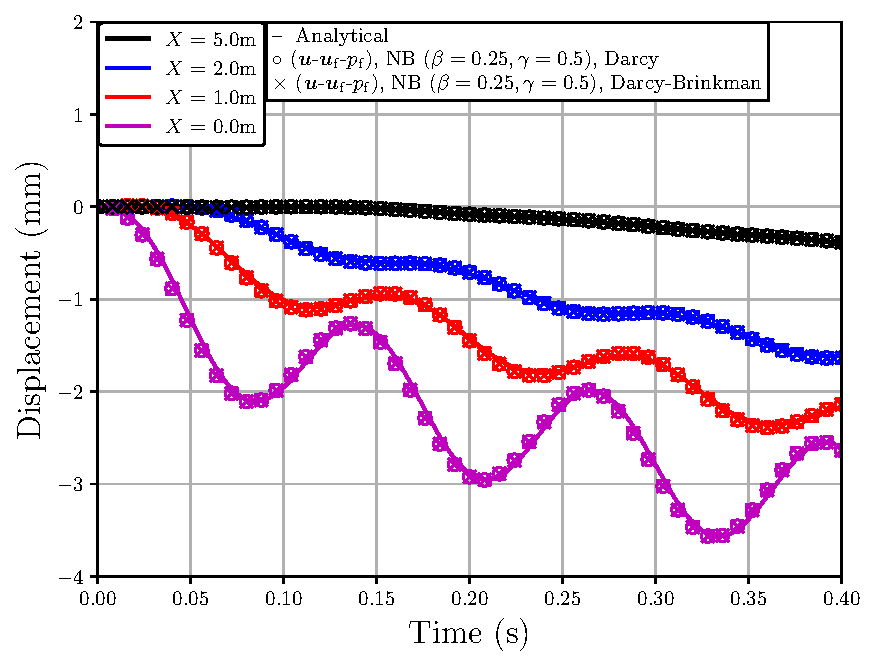
\includegraphics[width=0.45\textwidth]{./Cases/deBoer/figures/deBoer-disp-u.pdf}}
    \subfigure[format=hang][]{\label{fig:Examples_Verification_deBoer-disp-uf}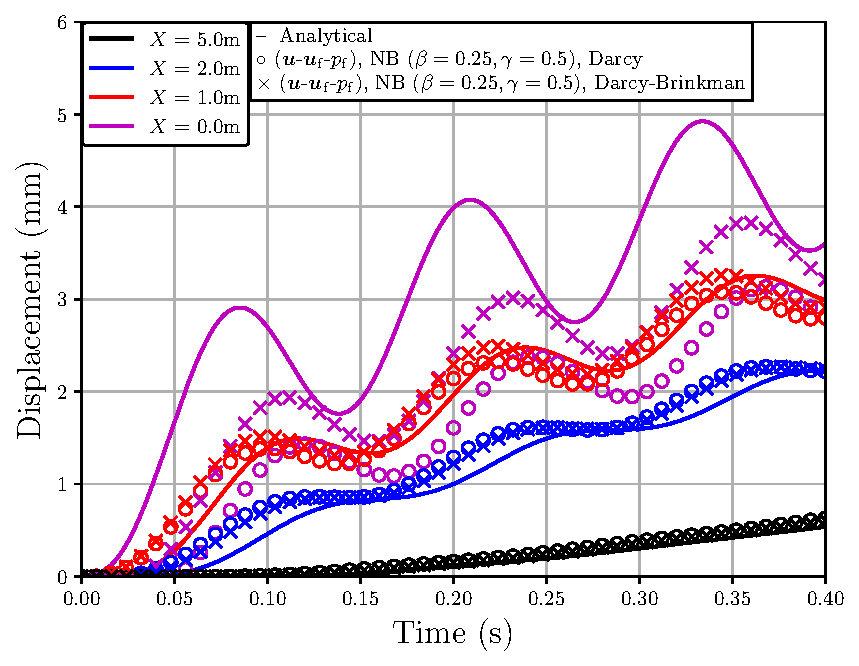
\includegraphics[width=0.45\textwidth]{./Cases/deBoer/figures/deBoer-disp-uf.pdf}}
    \newline
    \subfigure[format=hang][]{\label{fig:Examples_Verification_deBoer-press-PF}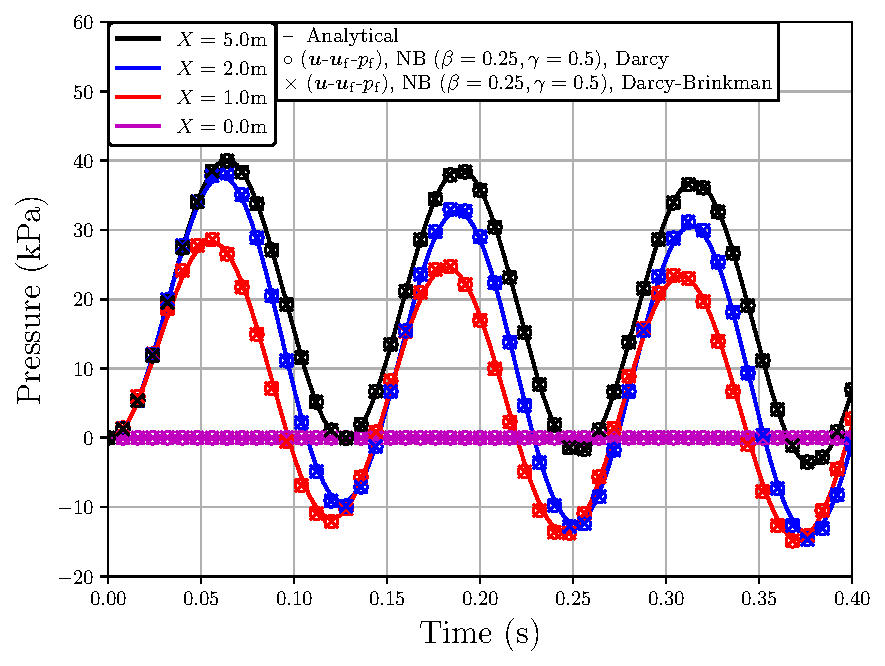
\includegraphics[width=0.45\textwidth]{./Cases/deBoer/figures/deBoer-press-PF.pdf}}
    \subfigure[format=hang][]{\label{fig:Examples_Verification_deBoer-stress}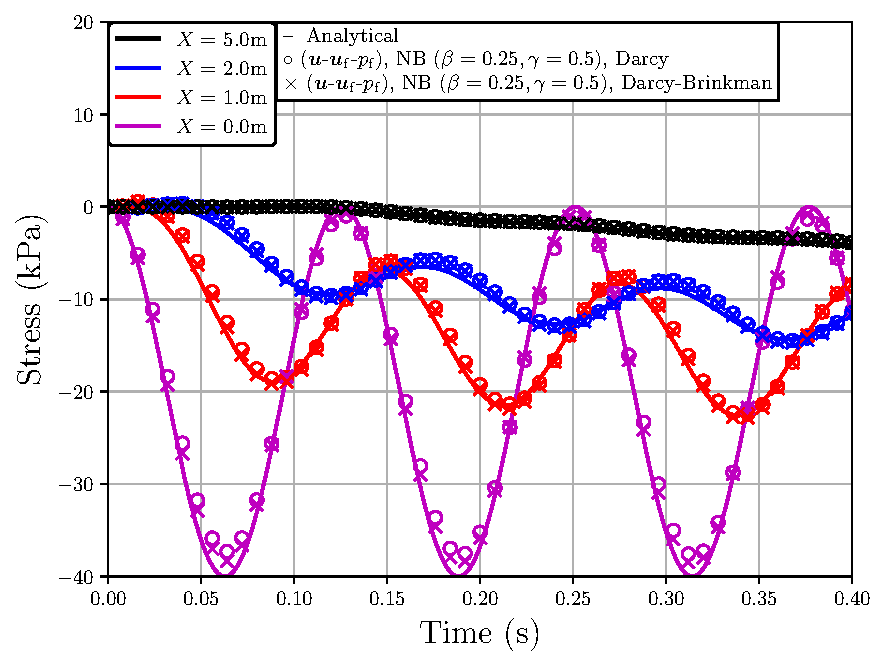
\includegraphics[width=0.45\textwidth]{./Cases/deBoer/figures/deBoer-stress.pdf}}
\caption{Verification results for the numerical approximation to the \citet{deBoer1993} analytical solution.}
\label{fig:Examples_Verification_deBoer-all}
\end{figure}
